








descobriu-se, para cada medida, qual configuração a otimiza. Os resultados completos estão disponíveis para consulta em~\urlsoftwares.



% --------------- --------------- ---------------
Analisou-se também o desempenho da mesma técnica aplicada a um texto contínuo extraído de artigo da Internet que descreve seis gêneros musicais brasileiros um após um outro separados em seções. Ao observar a Figura~\ref{fig:coesaolexicaTT-generos-musicais}, nota-se que os vales são mais definidos e a maioria dos segmentos coincidem ou estão próximos a segmentação de referência. A segmentação de referência possui sete segmentos que separam uma introdução do assuntos e respeitam cada uma das subseções que tratam de um gênero musical. Obtém-se nesse cenário uma eficiência maior em relação a segmentação da ata, o que sugere que textos organizados em seções podem ter melhores benefícios com técnicas baseadas em coesão léxica que as atas, onde esse fator é menos significativo.  % ou a premissa do algoritmo não é tão boa.



  %--- ---
  \begin{figure}[!h]
	  \centering
	  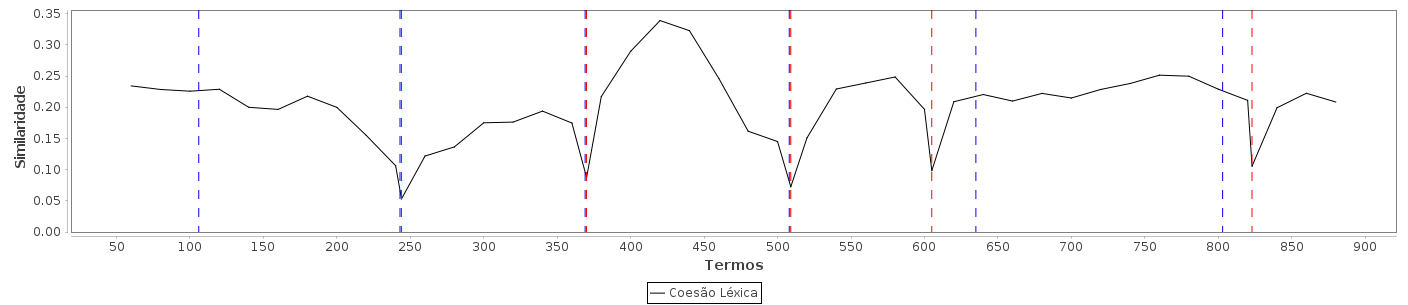
\includegraphics[width=\textwidth]{conteudo/capitulos/figs/generos-musicais-TT-40-20.png}
	  \caption{Variação da coesão léxica ao longo de um artigo melhor estruturado em seções junto a uma segmentação automática em contraste com uma segmentação de referência.}
	  \label{fig:coesaolexicaTT-generos-musicais}
  \end{figure}

% --------------- --------------- ---------------

  % De certa forma, tratar o C99 e o TT como pertencentes a mesma técnica = coesão léxica!!  % e depois justificar o por que de usar outras técnicas



% possuem parâmetros já otimizados configurados pelo desenvolvedor
% já testados por Mincut
% são afetados mais pela técnica que configuração de parâmetros 

% Obteve-se, para cada medida, 4 configurações, levando em conta ambos os algoritmos e a presença ou ausência do pré-processamento. Novamente utilizou-se o teste de Friedman e Nemenyi e descobriu-se, para cada medida, qual configuração a otimiza. Os resultados completos estão disponíveis para consulta em~\urlsoftwares.

Para os algoritmos \textit{TextTiling} e \textit{C99} 



sem aplicar o pré-processamento. 


com pós-teste de Nemenyi 

Inicialmente, calculou-se as medidas configurando cada algoritmo conforme mostrado na Subseção~\ref{subsec:configuracaoexperimental}, sem aplicar o pré-processamento. O teste de Friedman com pós-teste de Nemenyi foi utilizado para gerar um ranking das melhores configurações para cada medida calculada. Com isso, foi possível descobrir quais valores otimizam um algoritmo para uma medida, 	desconsiderando o pré-processamento. 

A fim de conhecer o impacto do pré-processamento, repetiu-se os testes com o texto pré-processado. Com isso, descobriu-se quais valores otimizam os algoritmos para cada medida, considerando essa etapa.

Com os testes anteriores obteve-se, para cada medida, 4 configurações, levando em conta ambos os algoritmos e a presença ou ausência do pré-processamento. Novamente utilizou-se o teste de Friedman e Nemenyi e descobriu-se, para cada medida, qual configuração a otimiza. Os resultados completos estão disponíveis para consulta em~\urlsoftwares.




\subsubsection{Resultados}


Obteve-se, por meio dos testes apresentados, as melhores configurações para as principais medidas de avaliação de segmentadores. Com essas configurações calculou-se a média de cada medida considerando o conjunto de documentos. 


A seguir são apresentados os resultados obtidos com os algoritmos baseados em coesão léxica, considerando seus principais parâmetros e a aplicação do pré-processamento. Em seguida, são apresentados os resultados da avaliação final dos algoritmos abordados nesse trabalho.


Na Tabela~\ref{tab:resultadosTT} são apresentadas, as médias obtidas com o \textit{TextTiling} bem como as configurações utilizadas, onde \textbf{J} é o tamanho da janela e \textbf{P} é o passo.


\begin{table}[!h]
	\centering
	\begin{tabular}{|l||c|c|c||c|c|c|} \hline

		& \multicolumn{3}{c||}{Sem Pré-processamento} 
		& \multicolumn{3}{c|}{Com Pré-processamento}\\			

		\textbf{Medida} & 
		\textbf{J} &
		\textbf{P} & 
		\textbf{Média} &
		\textbf{J} &
		\textbf{P} & 
		\textbf{Média} \\	\hline

		P$_k$				& 50 & 9 & 0,142 & 50 & 9  & 0,144 \\ \hline
		\textit{WindowDiff}	& 50 & 6 & 0,387 & 40 & 9  & 0,396 \\ \hline
		Acurácia			& 50 & 6 & 0,612 & 40 & 9  & 0,603 \\ \hline
		Precisão			& 40 & 9 & 0,611 & 50 & 12 & 0,613 \\ \hline
		Revocação			& 20 & 3 & 0,886 & 20 & 3  & 0,917 \\ \hline
		F$^1$				& 30 & 6 & 0,605 & 40 & 3  & 0,648 \\ \hline

	\end{tabular}
	\caption{Resultados obtidos com o \textit{TextTiling}}
	\label{tab:resultadosTT}
\end{table}




%%%%%%%%%%%%%%%%%%%%%%
% Análise da Coesão Léxica e eficiência da técnica do TT
%%%%%%%%%%%%%%%%%%%%%%

% --> Falar da coesão léxica peculiar das atas!!

Uma vez que a coesão léxica é pressuposto de muitas abordagens em segmentação textual, fez-se uma análise desses documentos quanto a similaridade dos termos ao longo do texto. Verificou-se que a técnica de janelas deslizantes empregada pelo TextTiling encontra os vales que indicam transições entre segmentos, contudo ao comparar esses vales com a segmentação de referência, nota-se que a maioria dos limites coincide  ou estão próximos aos vales, porém há casos onde a referência indica limites em trechos com alta coesão léxica e outros onde a queda da coesão, indicada por vales, não coincide com nenhum limite de referência. 



% Na Figura~\ref{fig:coesaolexicaTT}a linha horizontal representa a variação da coesão léxica ao longo de uma ata e as linha verticais azuis e vermelhas representam os limites entre segmentos atribuidos pela referência e pelo algoritmo respectivamente. 
Na Figura~\ref{fig:coesaolexicaTT} é apresentado a variação da coesão léxica ao longo de uma ata e a segmentação obtida pelo \textit{TextTiling} usando tamanho de janela igual a 50 e passo 9. A linha horizontal representa a variação da coesão léxica e as linha verticais azuis e vermelhas representam os limites entre segmentos atribuidos pela referência e pelo algoritmo respectivamente. 





  %--- ---
  \begin{figure}[!h]
	  \centering
	  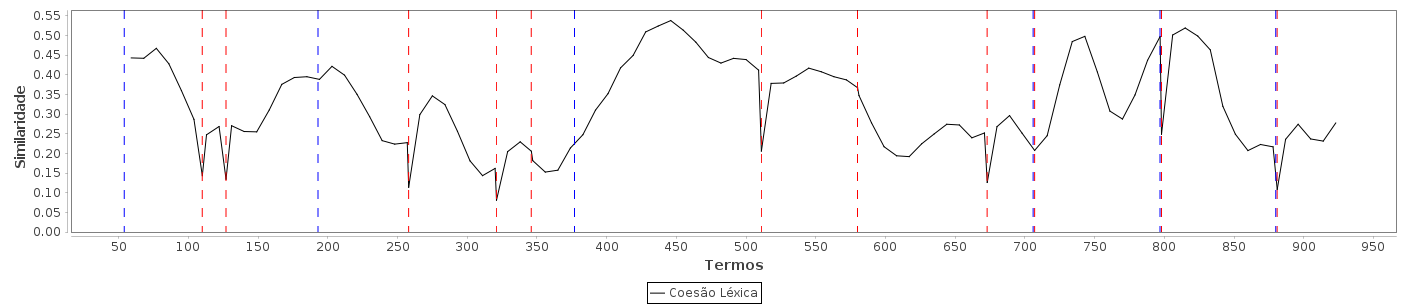
\includegraphics[width=\textwidth]{conteudo/capitulos/figs/coesaolexicaTT-50-9.png}
	  \caption{Variação da coesão léxica ao longo de uma ata junto a uma segmentação automática em contraste com uma segmentação de referência.}
	  \label{fig:coesaolexicaTT}
  \end{figure}


Analisou-se também o desempenho da mesma técnica aplicada a um texto contínuo extraído de artigo da Internet que descreve seis gêneros musicais brasileiros um após um outro separados em seções. Ao observar a Figura~\ref{fig:coesaolexicaTT-generos-musicais}, nota-se que os vales são mais definidos e a maioria dos segmentos coincidem ou estão próximos a segmentação de referência. A segmentação de referência possui sete segmentos que separam uma introdução do assuntos e respeitam cada uma das subseções que tratam de um gênero musical. Obtém-se nesse cenário uma eficiência maior em relação a segmentação da ata, o que sugere que textos organizados em seções podem ter melhores benefícios com técnicas baseadas em coesão léxica que as atas, onde esse fator é menos significativo.  % ou a premissa do algoritmo não é tão boa.



  %--- ---
  \begin{figure}[!h]
	  \centering
	  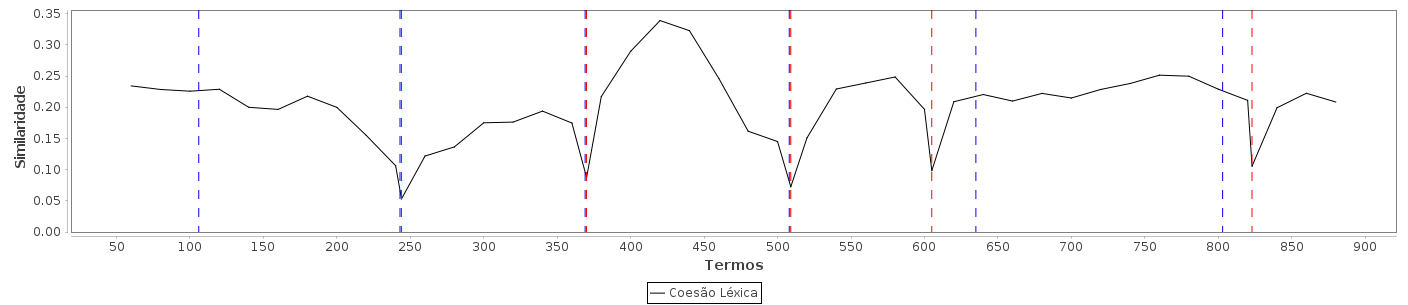
\includegraphics[width=\textwidth]{conteudo/capitulos/figs/generos-musicais-TT-40-20.png}
	  \caption{Variação da coesão léxica ao longo de um artigo melhor estruturado em seções junto a uma segmentação automática em contraste com uma segmentação de referência.}
	  \label{fig:coesaolexicaTT-generos-musicais}
  \end{figure}


  % De certa forma, tratar o C99 e o TT como pertencentes a mesma técnica = coesão léxica!!  % e depois justificar o por que de usar outras técnicas



Na Tabela~\ref{tab:resultadosc99} são apresentadas, as médias obtidas com o \textit{C99} bem como as configurações utilizadas, onde \textbf{S} é a proporção de segmentos em relação a quantidade de candidatos, \textbf{M} é o tamanho do quadro utilizado para criar a matriz de \textit{rankings} e \textbf{W} indica se os segmentos são representados por vetores contendo a frequência ou um peso das palavras.


\begin{table}[!h]
	\centering
	\begin{tabular}{|l||c|c|c|c||c|c|c|c|} \hline

		& \multicolumn{4}{c||}{Sem Pré-processamento} 
		& \multicolumn{4}{c|}{Com Pré-processamento}\\			

		\textbf{Medida} & 
		\textbf{S} & 
		\textbf{M} & 
		\textbf{W} & 
		\textbf{Média} &
		\textbf{S} & 
		\textbf{M} & 
		\textbf{W} & 
		\textbf{Média} \\	\hline

		P$_k$				& 20 & 9 & Sim & 0,134& 20 & 11 & False	& 0,116 \\ \hline  
		\textit{WindowDiff}	& 60 & 9 & Sim & 0,411& 60 &  9 & Sim 	& 0,390 \\ \hline  
		Acurácia			& 60 & 9 & Sim & 0,588& 60 &  9 & Sim 	& 0,609 \\ \hline  
		Precisão			& 40 & 9 & Sim & 0,645& 20 & 11 & False	& 0,720 \\ \hline  
		Revocação			& 80 & 9 & Sim & 0,869& 80 & 11 & Sim 	& 0,897 \\ \hline  
		F$^1$				& 80 & 9 & Sim & 0,638& 80 & 11 & Sim 	& 0,655 \\ \hline  

	\end{tabular}
	\caption{Resultados obtidos com o \textit{C99}}
	\label{tab:resultadosc99}
\end{table}



Verificou-se que o \textit{C99} obteve melhor desempenho em acurácia, precisão, $F^1$, $P_k$ e \textit{WindowDiff}, em relação ao \textit{TextTiling}, enquanto este obteve o melhor desempenho em revocação. De maneira geral, o algoritmo \textit{C99} apresenta melhores resultados em relação ao \textit{TextTiling}, contudo testes estatísticos realizados indicaram que não houve diferença significativa entre os métodos. 



% --> Fechar falando sobre os métodos baseados em coesão léxica.


% --> Fechar falando sobre os métodos baseados em coesão léxica.


A avaliação final foi feita pela comparação dos algoritmos usando as medidas \textit{Pk} e \textit{WindowDiff}. É apresentada também, para fins de comparação, as medidas tradicionais acurácia, precisão, revocação e F$^1$, entretanto, nesse contexto, essas medidas são menos significativa que Pk e WindowDiff, conforme já mencionado na Seção~\ref{xx}. A Tabela~\ref{tab:configfinal} contém as médias com cada algoritmo. Vale lembrar que P$_k$ e \textit{WindowDiff} são medidas de dissimilaridade, ou seja, os valores menores significam melhores resultados.

\begin{table}[!h]
	\centering
\begin{tabular}{|l||c|c|c|c|c|c|c|} 
\hline 
\textbf{M\'{e}todo} & 
\textbf{Pk} & 
\textbf{WD} & 
\textbf{A } & 
\textbf{P } & 
\textbf{R } & 
\textbf{F1} & 
\textbf{Segmentos}\\ \hline

Senten\c{c}as & 0.320 & 0.502 & 0.498 & 0.498 & \textbf{1.000} & \textbf{0.642} & 22.083\\ \hline
TextTiling    & 0.275 & 0.469 & 0.531 & 0.514 & 0.937 & 0.640 & 19.583\\ \hline
C99           & 0.142 & 0.426 & 0.574 & 0.601 & 0.473 & 0.506 & 8.167\\ \hline
BayesSeg      & 0.148 & 0.414 & 0.586 & 0.599 & 0.526 & 0.528 & 8.750\\ \hline
MinCut        & 0.226 & 0.532 & 0.468 & 0.464 & 0.438 & 0.432 & 10.333\\ \hline
TextSeg       & \textbf{0.085} & \textbf{0.387} & \textbf{0.613} & \textbf{0.714} & 0.412 & 0.497 & 5.167\\ \hline
\end{tabular} 

	\caption{Melhores resultados obtidos.}
	\label{tab:configfinal}
\end{table}


Na Figura~\ref{fig:grafico-medidas-tradicionais} é apresentada a performance dos algoritmos nas medidas tradicionais. Observa-se valores altos de revocação para a segmentação por sentenças, pois é atribuído um limite a todo candidato a final de segmento, o que resulta no valor máximo para revocação. De maneira semelhante, o comportamento do \textit{TextTiling} gera 
mais segmentos em relação aos demais, e com isso tem-se valores maiores de revocação, o que pode ser contornado configurando o algoritmo com passos maiores, ou ainda, sobre-escrevendo a função que calcula os \textit{depth scores} para reconhecer vales mais largos.

%--> TODO: explicar (a conceituação teórica) que passos curtos geram mais segmentos

  \begin{figure}[!h]
	  \centering
	  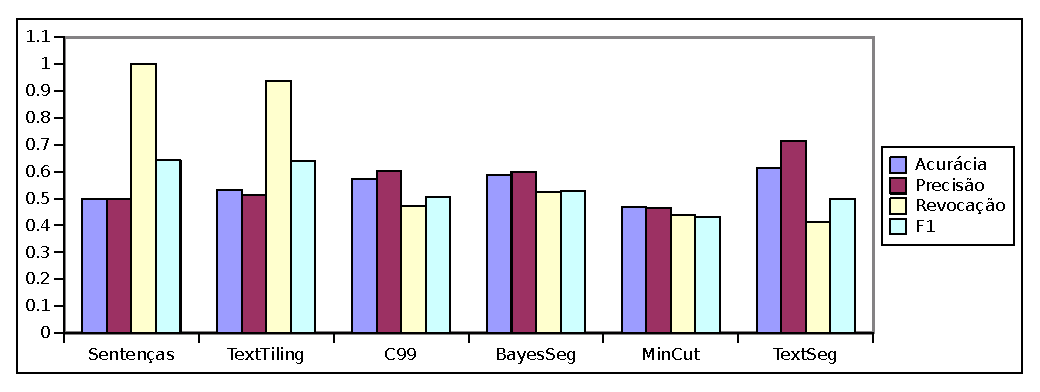
\includegraphics[width=1\textwidth]{conteudo/capitulos/figs/grafico-medidas-APRF1.eps}
	  \caption{Performance dos algoritmos de segmentação textual com as medidas tradicionais}
	  \label{fig:grafico-medidas-tradicionais}
  \end{figure}
  

Na Figura~\ref{fig:grafico-medidas-Pk-Wd} é apresentada a performance dos algoritmos nas medidas P$_k$ e \textit{WindowDiff}. Verifica-se que \textit{TextSeg} apresenta valores de \textit{WindowDiff} próximas ao \textit{C99} e \textit{BayesSeg} e resultados mais significantes quando medidos por P$_k$ em relação aos demais algoritmos.



  \begin{figure}[!h]
	  \centering
	  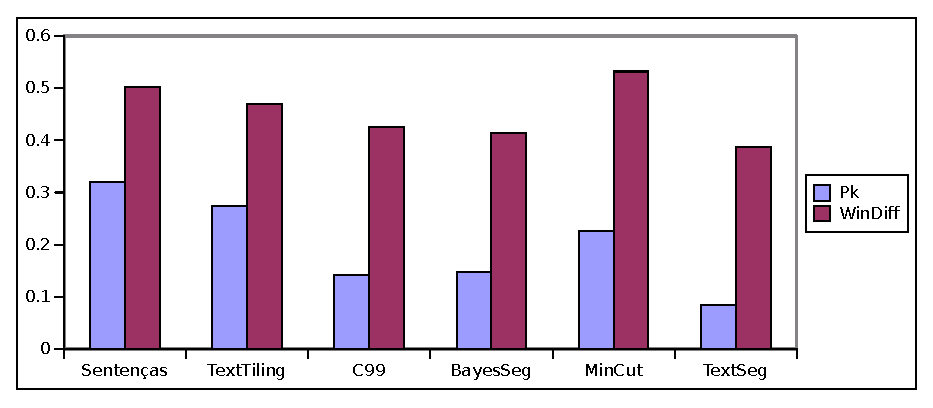
\includegraphics[width=1\textwidth]{conteudo/capitulos/figs/grafico-medidas-Pk-Wd.eps}
	  \caption{Performance dos algoritmos de segmentação textual com as medidas P$_k$ e \textit{WindowDiff}.}
	  \label{fig:grafico-medidas-Pk-Wd}
  \end{figure}












% cada segmento é um documento
Após a identificação dos segmentos, o algoritmo retorna uma lista onde cada elemento é um texto com um assunto predominante e será a partir de disso considerado um documento.

% -? Medidas

% -- como ele faz?




%  ==========   ==========   ==========   ==========   ==========   

\subsection{Representação Computacional}

As etapas anteriores produzem fragmentos de documentos onde o texto esta em um estágio de processamento inicial, com menos atributos que as versões originais, onde cada fragmento está associado a um tema, porém, ainda não estruturado. Ocorre que as técnicas de mineração de texto exigem uma representação estruturada dos textos. % conforme será visto na Seção~\ref{subsection:RepTextos}.

Uma das formas mais comuns é a representação no formato matricial conhecida como Modelo Espaço Vetorial (\textit{Vectorial Space Model} - VSM)~\cite{Rezende2003}, onde os documentos são representados como vetores em um espaço Euclidiano $t$-dimensional em que cada termo extraído da coleção é representado por um dimensão. Assim, cada componente de um vetor expressa a relação entre os documentos e as palavras. Essa estrutura é conhecida como \textit{document-term matrix} ou matriz documento-termo.  Nesse trabalho a representação empregada é a \textit{Bag Of Words} a qual sintetiza a base de documentos em um contêiner de palavras, ignorando a ordem em que ocorrem, bem como pontuações e outros detalhes, preservando apenas o peso de determinada palavra nos documentos. 



% --> \subsection{Extração de Tópicos}

% a tarefa é identificar qual assunto está presente em cada trecho e qual é o tipo de ocorrência.



\section{Módulo Consulta}

Uma vez que a estrutura de dados interna contem os assuntos abordados na coleção de documentos, o tipo de ocorrência para cada assunto e o trecho onde se encontram, caberá ao módulo de consulta receber a \textit{string} de consulta do usuário, resgatar os dados desejados e apresentá-los em ordem cronológica, dando condições para o usuário acessar os segmentos encontrados bem como os documentos originais.

% \subsection{Seleção dos tópicos}

\subsection{Visualização}

O usuário final precisa de uma interface adequada para visualizar os resultados da busca considerando-se a relevância dos tópicos selecionados e a sequência cronológica. Uma boa apresentação deve permitir ao usuário identificar a relevância os resultados e ser relativante independente para compreensão do conteúdo, evitando a leitura do texto completo. Ou seja, o texto de cada tópico apresentado deve ser suficiente para compreensão do assunto mencionado, sem necessidade de visualizar o documento original.

As informações apresentadas, incluem dados obtidos do documento como o nome do arquivo, e o texto onde o assunto é mencionado. Além disso, apresenta-se as informação extraídas pelas técnicas de mineração de texto como os descritores e rótulos. Para cada busca, é retornada uma lista de resultados ordenados pela relevância com a \textit{string} de entrada, sendo cada item referente a uma menção a um assunto. Um tópico é abordado em diferentes momentos e registrado em atas distintas, onde cada menção é um resultado a ser apresentado. 

Como parte da proposta, o sistema apresenta cada resultado dentro de um histórico de menções. Para isso, abaixo do texto é exibida uma linha com links para os resultados que compartilham o mesmo tópico ordenados por data. Os links, ao ser acionado, direciona para o resultado que aponta, além disso, quando o cursor do mouse está sobre o link, é apresentado um pre-visualização do texto. Dessa forma o usuário tem acesso uma interface que lhe fornece uma visão temporal das menções.


% Uma vez que um item faz menção a um tópico específico, 
% o sistema traz vários resultados para uma consulta, alguns mais relevantes que outros. Para cada resultado (que podem tratar de coisas diferentes) o sistema apresenta um histórico de menções para aquele assunto;


% \section{Estudo de caso}
% -- qual o ganho em relação a um sitema de busca por palavras-chave? 


% --> \section{Avaliação}
















---------------------------------------------------------------------------------




O \textit{C99}, assim como outros métodos baseados em divisão, tem sua performance fortemente influenciado pela quantidade segmentos desejados. Esses métodos alcançam melhores resultados em contextos onde a quantidade de segmentos é conhecida~\cite{Bokaei2015,Ferret2009,Kern2009,Naili2016}. Na Figura~\ref{fig:influencia-NSegs-WD} é mostrado a variação de \textit{WindowDiff} em função da quantidade de segmentos solicitada ao algoritmo. Observa-se que há um ponto ótimo próximo 0,45 indicando que para o conjunto de atas analisado o método dá melhores resultados com número de segmentos desejados próximo a 45\% do número de sentenças.

  \begin{figure}[!h]
	  \centering
	  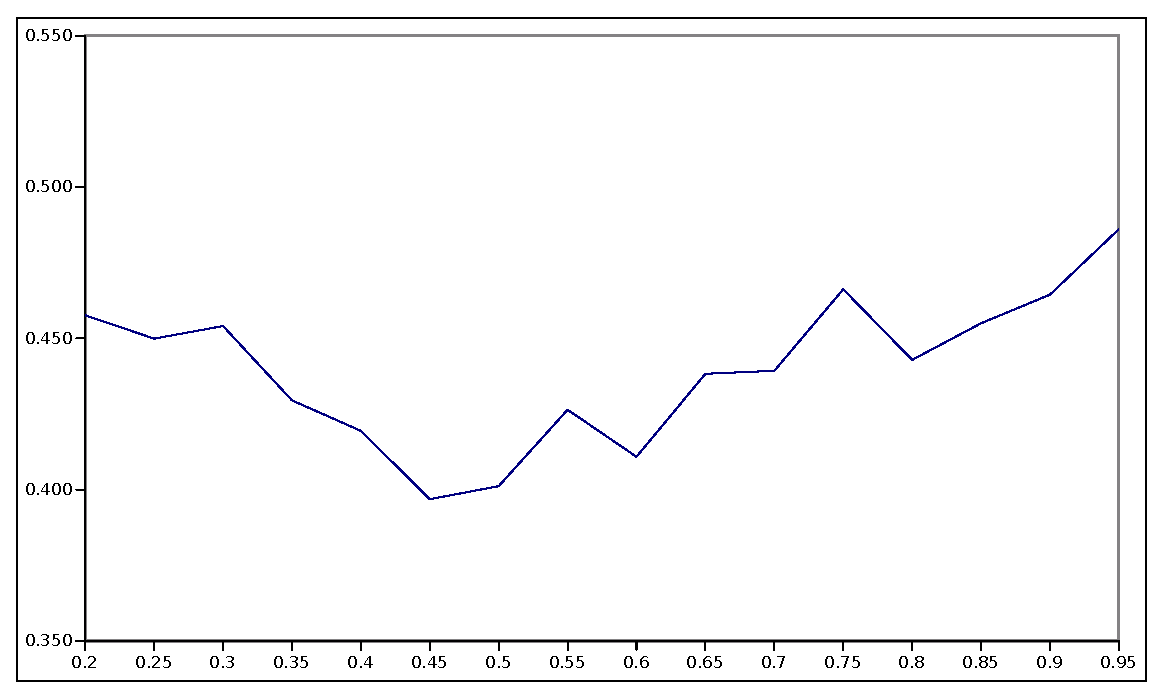
\includegraphics[width=0.9\textwidth]{conteudo/capitulos/figs/influencia-qtd-Segs-WD-C99.eps}
	  \caption{Influência da quantidade de segmentos em \textit{WindowDiff}}
	  \label{fig:influencia-NSegs-WD}
  \end{figure}






















